\documentclass[a4paper,11pt]{article}
\title{\textbf{Project DiSA (Digitally Signed Archive)}}
\author{
    André Cardoso,\\
    andremacardoso@ua.pt,\\
    108269\\
    \and
    Bruno Páscoa,\\
    brunopascoa03@ua.pt,\\
    107418\\
    \and
    Maria Sardinha,\\
    mariasardinha@ua.pt,\\
    108756\\
    \and
    Miguel Pinto,\\
    miguel.silva48@ua.pt,\\
    107449\\
    \and
    Pedro Rei,\\
    pedrorrei@ua.pt,\\
    107463\\
    \and  
    Tiago Figueiredo,\\
    tiago.a.figueiredo@ua.pt,\\
    107263\\
    \and
    Advisor Teachers,\\
    José Vieira \& André Zúquete\\
}

\date{\today}

%packages
\usepackage[utf8]{inputenc}
\usepackage{graphicx}
\usepackage{listings}
\usepackage{xcolor}
\usepackage{microtype}
\usepackage{xspace}
\usepackage{url}
\usepackage{csquotes}
\usepackage{lipsum}
\usepackage{hyperref}
\usepackage[
    backend=bibtex,
    style=alphabetic,
    sorting=ynt,
    bibencoding=utf8
]{biblatex}
\addbibresource{project1.bib}

\fontsize{11pt}{13pt}\selectfont
\setlength\parindent{11pt}
\definecolor{dkgreen}{rgb}{0,0.6,0}
\definecolor{mauve}{rgb}{0.58,0,0.82}
\definecolor{gray}{rgb}{0.5,0.5,0.5}
\lstset{basicstyle=\ttfamily,
    showstringspaces=false,
    commentstyle=\color{dkgreen},
    keywordstyle=\color{blue},
    columns=flexible,
    basicstyle={\small\ttfamily},
    numbers=left,
    numberstyle=\tiny\color{gray},
    stringstyle=\color{mauve},
    breaklines=true,
    breakatwhitespace=true,
}

% Adjusting table of contents
\setcounter{secnumdepth}{3}
\setcounter{tocdepth}{3}

% Document
\begin{document}
    \begin{figure}
        \centering
        
\includegraphics[width=0.9\textwidth]{images/deti.png}\label{fig:figure}
    \end{figure}
    \maketitle
    \clearpage
    \tableofcontents
    \clearpage
    \clearpage
    \section{Abstract}\label{sec:Abstract}
        \quad In the digital age, the demand for efficient document submission faces persistent challenges due to storage limitations and file upload constraints. To face these obstacles, our project seeks to develop an innovative digital document archiving platform, dedicated to redefine document management with a commitment to authenticity (using a blockchain) and integrity (through digital signatures).

        The signatures of documents to be submitted are made on client's side, with their citizen card or digital mobile key (thus guaranteeing the identity of the author). Please note that one or more documents can be submitted, and they will always be collected in a .tar file.

        These signatures are, then, used to generate a manifest whose hash is sent to an external blockchain (Polygon PoS \cite{PolygonPos}) and the file is archived using Paperless \cite{Paperless} (initially it was planned to use Archivematica \cite{Archivematica}, but we decided to change due to problems with the service).

        The use of a blockchain (and, in particular, a blockchain over which we have no influence) is the proof of existence of the documents, as it allows to guarantee the date and value of the stored hash, which can be compared with the hash of the manifest (automatically via the browser, or manually via the tracker link provided) in order to verify its authenticity.

        After submitting documents, it is then possible to view and manage the submitted documents, as well as share them (based on white-listing) in which any user, with whom the collection (set of files) is shared, will be able to download the content and proof of existence (manifest), all on a website developed for this purpose.

        In general, the system consists of two user interfaces (submission in an application separated from the collection management and sharing website), as well as blockchain service, back-office for processing all requests, and also the chosen file system (Paperless).

        With all this, DiSA's main use cases would be in the storage of documents whose authenticity and integrity guarantees are imperative, such as legal or government documents, companies, and artists (in order to preserve they intellectual property).

        Supported by the Library and STIC services at the University of Aveiro, our effort aims to address digital document management's problems, empowering users with a secure, efficient, and user-friendly digital document archival solution, backed by authenticity guarantee.

        \vspace{0.5cm}
        \textbf{Keywords:} Digital Document Archiving, Document Authenticity, Documents, Digital Signatures, Blockchain Technology, Streamlined Submission Process, Unique Document Referencing, Paperless Integration, User-friendly Interface, Document Management

    \clearpage
    \section{Introduction}\label{sec:intro}
        \quad In this section, we will provide an overview of the project, including the context, motivation, goals, expected results, and the structure of the document. This will set the stage for understanding the importance and relevance of our work.
    
        \subsection{Context}
            \quad In today's digital landscape, organizations across diverse sectors are embracing digitization to streamline operations and enhance efficiency. This shift towards digital processes has led to a proliferation of digital documents, ranging from reports and contracts to research papers and administrative records.
            
            However, the growing quantity of digital documents presents challenges. Storage limitations become pressing as the volume of documents increases, with public institutions facing significant hurdles due to restricted capacities and stringent upload restrictions imposed by digital platforms. Additionally, ensuring the authenticity and integrity of digital documents is crucial, as digital manipulation becomes easier, making verification complex, especially in legal or academic contexts.
            
            Addressing these challenges demands innovative solutions that provide ample storage, seamless document handling, and robust authentication mechanisms. Our project, DiSA (Digital Signed Archive), aims to develop a cutting-edge digital document archiving platform leveraging advanced technologies and user-centered design to revolutionize document management.       
            
        \subsection{Motivation}
            \quad The motivation for DiSA stems from the need to address the challenges posed by digitizing document management. As organizations transition to digital processes, the volume of digital documents grows exponentially, presenting critical issues.
    
            Traditional storage methods are insufficient for the vast quantities of digital documents generated. Organizations, especially public institutions, face storage capacity constraints and file upload limitations. There is a need for scalable and cost-effective storage solutions.
            
            Ensuring the authenticity and integrity of digital documents is a significant concern. Verifying the credibility of documents has become challenging due to the ease of digital manipulation. Robust mechanisms are needed to authenticate the origin and integrity of digital documents.

            \pagebreak
            Moreover, the process of handling and managing digital documents needs to be efficient. Users require intuitive platforms for document submission, retrieval, and verification. Integration with existing platforms enhances accessibility and usability.
            
            By addressing these challenges, DiSA aims to revolutionize digital document management, providing tools and functionalities for secure storage, authentication, and management of digital documents.
    
        \subsection{Goals}
            Our project aims to achieve the following goals:
    
            \begin{itemize}
             \item \textbf{1. Simplify Document Submission:} Develop an intuitive user interface for quick and secure document uploads to be done by users of any age or background.
            
             \item \textbf{2. Guarantee Authenticity and Integrity:} Use digital signatures and blockchain technology to prevent tampering of already submitted documents.
    
             \item \textbf{3. Scalable Storage:} Provide a scalable storage solution for large documents and big number of users.
    
             \item \textbf{4. Seamless Access and Retrieval:} Ensure easy access and retrieval of documents by any allowed user.
    
             \item \textbf{5. Enhanced Security and Privacy:} Implement robust security measures and access control policies.
    
             \item \textbf{6. Interoperability and Compatibility:} Ensure seamless integration with existing systems and standards.

             \item \textbf{7. Auditing and Version Control:} Implement mechanisms for tracking document history and verifying authenticity.
            \end{itemize}
            
        \subsection{Expected Results}
            We anticipate the following outcomes from our project, reflecting the successful achievement of our interconnected goals:
    
            \begin{itemize}
             \item \textbf{1. Enhanced User Experience:} Streamlined and efficient document submission process, resulting in increased user satisfaction and engagement. 
            
             \item \textbf{2. Improved Document Security:} Enhanced document security through digital signatures and blockchain technology.
    
             \item \textbf{3. Scalable Storage Solution:}  Ability to archive large volumes of data with minimal constraints to the end-users.
    
             \item \textbf{4. Easy Access and Retrieval:} Seamless access to archived documents for users and organizations, also facilitating their share-ability.
    
             \item \textbf{5. Enhanced Security and Privacy:} Implement robust security measures and access control policies.
    
             \item \textbf{6. Enhanced Interoperability:} High compatibility with existing systems ans standards.

             \item \textbf{7. Transparent Document History:} Guaranteed accessibility and integrity of documents, along with their various versions over time.
            \end{itemize}
    
        \subsection{Document Structure}
        This report is organized as follows:
        \begin{itemize}
            \item \textbf{State of the Art}: A review of existing solutions and related work in the domain of document archiving and digital signatures.
            \item \textbf{Product Concept}: Detailed system requirements, including functional and non-functional requirements, use cases, and system architecture.
            \item \textbf{Implementation}: Description of the implementation process, covering the presentation, authentication, business, storage, and integrity layers.
            \item \textbf{Project Management}: An overview of team roles and communication plans.
            \item \textbf{Conclusions and Future Work}: Summary of the main results, discussion of limitations, and suggestions for future improvements.
        \end{itemize}
    
    \clearpage
    \section{State of the Art}\label{sec:soa}

        \subsection{Introduction}
        \quad In this section, we'll provide an overview of current technologies and solutions relevant to our project. Reviewing existing work is essential because it helps us understand what's already out there, what works well, and what could be improved.

        By looking at similar projects and technologies, we can identify gaps and opportunities for innovation in our own project. This helps us ensure that our solution is not only effective but also unique.
        
        We'll cover areas like document archive platforms, digital signature platforms, and other notable solutions. This review will highlight important insights that guide our design and implementation choices, making sure our project stays up-to-date with the latest advancements in the field.
        
        \subsection{Related Work}
            \quad In our exploration of existing solutions in the field of digital document management and signatures, we identified several notable platforms and technologies that will be detailed below.
        
            \subsubsection{Document Archive Platforms}
            \begin{itemize}
                \item \textbf{DSpace \cite{DSpace}}: An open-source repository commonly used by academic institutions to manage and store various types of documents such as datasets, theses, and images.
                
                \item \textbf{Archivematica}: An open-source platform focused on the preservation of digital content, offering comprehensive tools to manage and preserve digital archives, ensuring their long-term accessibility and integrity.
                
                \item \textbf{Preservica \cite{Preservica}}: A paid platform that supports multiple formats, including images and videos, used by institutions requiring long-term storage and preservation of documents.
                
                \item \textbf{Paperless}: An open-source platform for secure and permanent document storage, providing features for organizing and preserving documents to ensure their accessibility and integrity over time.
            \end{itemize}
    
        \subsubsection{Digital Signature Platforms}
        \begin{itemize}
            \item \textbf{Blockcerts \cite{Blockcerts}}: An open standard that uses blockchain technology to issue and verify digital certificates. However, it relies on the existence of an issuing institution.
            
            \item \textbf{Proof of Existence \cite{ProofOfExistence}}: A platform that enables users to submit a document's hash onto the Bitcoin blockchain, providing proof of the document's existence at a specific point in time. It is available as both a standalone platform and an npm package.
        \end{itemize}
        
        \subsubsection{Other Notable Solutions}
            \begin{itemize}
            \item \textbf{JSign \cite{JSign}}: A solution for digitally signing documents using blockchain technology, although limited to a web-based service.
            
            \item \textbf{DocuSign \cite{DocuSign}}: A leading player in the eSignature market, focusing primarily on electronic signatures. However, it lacks integrated support for blockchain-based authentication.
        \end{itemize}

        \subsection{Conclusions}
            \quad While these solutions excel in specific areas of document management, none fully integrate both digital signatures and blockchain technology into a unified platform like DiSA aims to do. By combining the strengths of these technologies, DiSA seeks to provide organizations with a comprehensive solution for secure, authentic, and long-term document management.

    \clearpage
    \section{Product Concept}\label{sec:productconcept}

        \subsection{Overview}
        \quad The DiSA (Digitally Signed Archive) platform aims to revolutionize digital document management by providing scalable storage, seamless document handling, and robust authentication mechanisms. Our platform is designed to address the critical challenges of digital document storage, authenticity, and integrity, offering a comprehensive solution for organizations and users across various sectors.
        
        \subsection{System Requirements}    
    
            \subsubsection{Requirements Elicitation}
                The requirements elicitation process involved gathering and defining the needs and constraints of all stakeholders to ensure that the final system meets their expectations and business needs. This process included:
        
                \begin{itemize}
                    \item \textbf{Stakeholder Meetings:} Conducting meetings with stakeholders (our advisors) to understand their needs, expectations, and challenges.
        
                    \item \textbf{Workshops:} Participating in a presentation to gain insights of a document management platform used in a previous project, Archivematica, where the presenter was Rafael Direito.
        
                    \item \textbf{Brainstorming Sessions:} Organizing brainstorming sessions among group members and advisors to define and prioritize requirements.
        
                    \item \textbf{Analysis of Existing Systems:} Reviewing current document management and digital signature systems to identify gaps and opportunities for improvement.
        
                    \item \textbf{Use Case Scenarios:} Developing use case scenarios to illustrate how different users will interact with the system. 
                \end{itemize}
            
            \subsubsection{Context}
                \quad The system operates in a digital environment where organizations need efficient and secure document management solutions. This includes integrating with existing platforms and ensuring compliance with regulatory requirements.

            \pagebreak
            \subsubsection{Actors}
            We identified the different types of users or entities that will interact with the system:
                \begin{itemize}
                    \item \textbf{Administrators:} Manage the system by analyzing auditing output of user interactions and maintain overall system health.
                    
                    \item \textbf{End Users:} Upload, retrieve, share and manage their documents within the system.
                    
                    \item \textbf{Third-Party Services:} Provide extra functionality, such as authentication (e.g. Autenticação.gov \cite{AutenticacaoGov}) or integrity services (e.g. blockchain integration).
                \end{itemize}
            
        
            \subsubsection{Use Cases}
            \quad Each use case describes the interactions between actors and the system to achieve specific goals. In each one we will detail the steps involved and the expected outcomes.
            
                \begin{itemize}
                    \item \textbf{Use Case 1 - Document Submission}
                    \begin{itemize}
                        \item \textbf{Actor}: John Smith (document submitter)
                        \item \textbf{Motivation}: John wants to store his application documents in a secure and trustworthy way.
                        \item \textbf{Preconditions}: John is authenticated in the system and owns a digital document ready for submission.
                        \item \textbf{Actions}:
                        \begin{enumerate}
                            \item John selects the documents to be submitted.
                            \item The system requests the digital signature of the documents.
                            \item John digitally signs the documents.
                            \item The system processes the documents and uploads them.
                            \item The system generates a receipt linking original and processed documents (through hash) containing a unique link.
                            \item The system stores the receipt's hash in the blockchain (and should be accessible by John).
                            \item John can now share and/or save the unique link obtained (and its receipt).
                        \end{enumerate}
                        \item \textbf{Post-conditions}: The documents are stored securely and authenticated with a unique unique link for access and validation.
                    \end{itemize}

                    \pagebreak
                    \item \textbf{Use Case 2 - Document Retrieval}
                    \begin{itemize}
                        \item \textbf{Actor}: Emily Davis
                        \item \textbf{Motivation}: Emily wants to retrieve a document (a teacher's application).
                        \item \textbf{Preconditions}: Emily has a unique link (given by the system).
                        \item \textbf{Actions}:
                        \begin{enumerate}
                            \item Emily accesses the system using the unique link.
                            \item The system verifies the link's authenticity (if it is valid and exists) and Emily's permission to access the document.
                            \item The system recovers the documents associated with the link given.
                            \item The system provides the document(s) to Emily, allowing visualization/download.
                        \end{enumerate}
                        \item \textbf{Post-conditions}: Emily has access to visualize/download the documents while being assured they are authentic and untampered with. (Note: Sometimes the document cannot be accessed until a certain date - embargoed state)
                    \end{itemize}
                    
                    \item \textbf{Use Case 3 - Document Update}
                    \begin{itemize}
                        \item \textbf{Actor}: John Smith
                        \item \textbf{Motivation}: John wants to update his previously submitted documents.
                        \item \textbf{Preconditions}: John is authenticated and has permission to update the document.
                        \item \textbf{Actions}:
                        \begin{enumerate}
                            \item John selects the document to be updated.
                            \item The system asks for the digital signature of the new version of the document.
                            \item John signs the new version of the document.
                            \item The system validates the digital signature and records the new version of the document's hash on the blockchain.
                            \item The system updates the unique link to point to the new version of the document.
                            \item The system confirms the update and displays the updated unique link.
                        \end{enumerate}
                        \item \textbf{Post-conditions}: The document is securely updated, and the unique link reflects the most recent version of the document.
                    \end{itemize}

                    \pagebreak
                    \item \textbf{Use Case 4 - Document Sharing}
                    \begin{itemize}
                        \item \textbf{Actor}: John Smith
                        \item \textbf{Motivation}: John wants to share his submitted documents.
                        \item \textbf{Preconditions}: John is authenticated and has permission to share the document.
                        \item \textbf{Actions}:
                        \begin{enumerate}
                            \item John selects the document to be shared.
                            \item The system requests John’s authentication to confirm permission.
                            \item The system allows John to share the document by white-listing an email address.
                        \end{enumerate}
                        \item \textbf{Post-conditions}: The document is shared to the corresponding email address as requested by John.
                    \end{itemize}
                    
                    \item \textbf{Use Case 5 - Document Change Tracking}
                    \begin{itemize}
                        \item \textbf{Actor}: Emily Davis
                        \item \textbf{Motivation}: Emily wants to track the changes made to a document received through a unique link.
                        \item \textbf{Preconditions}: Emily has a unique link to a document and wants to track its changes. She should also have permission by the owner to do so.
                        \item \textbf{Actions}:
                        \begin{enumerate}
                            \item Emily inserts the unique link in the system.
                            \item The system searches for the document in the system
                            \item The system the verifies if Emily should have access to its change history.
                            \item The system displays the change history.
                        \end{enumerate}
                        \item \textbf{Post-conditions}: Emily has access to the document’s change history, allowing her to track the changes over time.
                    \end{itemize}
                            
                    \item \textbf{Use Case 6 - System Auditing}
                    \begin{itemize}
                        \item \textbf{Actor:} Administrator
                        \item \textbf{Motivation:} The administrator wants to audit user activities and system operations for security and compliance purposes.
                        \item \textbf{Preconditions:} The administrator is authenticated and has the necessary permissions.
                        \pagebreak
                        \item \textbf{Actions:}
                        \begin{enumerate}
                            \item The administrator accesses the system audit logs.
                            \item The system retrieves and displays user activities and system events.
                            \item The administrator reviews the logs for any anomalies or compliance issues.
                            \item If necessary, the administrator takes corrective actions based on the audit findings.
                        \end{enumerate}
                        \item \textbf{Post-conditions:} The system remains secure and compliant with organizational policies, and any issues are addressed.
                    \end{itemize}
                \end{itemize}

                \textbf{Note:} Third-party services, such as authentication and integrity services, influence all use cases by providing essential functionalities like verifying user identities and ensuring document integrity.
    
            \subsubsection{Functional Requirements} \label{sec:fun-requirements}
            \quad Functional requirements describe the specific behaviors and functions that the system must perform, directly supporting the system's primary objectives. We found the main ones to be:
            
                \begin{itemize}
                    \item \textbf{Document Submission:} 
                    \begin{itemize}
                        \item The system must allow users to submit individual documents or sets of documents.
                        \item The system must support large document sizes, up to 100MB.
                    \end{itemize}
                    
                    \item \textbf{Authenticity Guarantee:} 
                    \begin{itemize}
                        \item The system must implement digital signatures to ensure authenticity of submitted documents.
                        \item The system must prevent changes to documents after submission without changing their timestamp.
                        \item Users must be able to verify the authenticity of documents at any time.
                    \end{itemize}
                    
                    \item \textbf{Proof of Existence:} 
                    \begin{itemize}
                        \item The system must incorporate a mechanism to prove the existence of a document at a given time, using blockchain integration or similar technology.
                    \end{itemize}

                    \pagebreak
                    \item \textbf{Document Sharing:} 
                    \begin{itemize}
                        \item The system must generate a unique link for each document or set of documents, allowing for easy reference and verification of authenticity.
                    \end{itemize}
                    
                    \item \textbf{Persistence Archive:} 
                    \begin{itemize}
                        \item The system must integrate with an archival platform to ensure long-term preservation and accessibility of documents.
                    \end{itemize}
                    
                    \item \textbf{User Interface:} 
                    \begin{itemize}
                        \item The system must feature an intuitive and user-friendly interface that prioritizes ease of use and accessibility for all users.
                    \end{itemize}
                    
                    \item \textbf{Receipt Generation:} 
                    \begin{itemize}
                        \item The system must automatically generate a receipt for each submitted document, linking the downloadable document to its submitted counterpart for authenticity verification.
                    \end{itemize}
                \end{itemize}
        
            \subsubsection{Non-Functional Requirements}
            \quad Non-functional requirements define the system's quality attributes, such as performance, security, and usability, ensuring it meets user expectations and operates efficiently and reliably. Below there is a list of those we found most relevant:
        
                \begin{itemize}
                    \item \textbf{Performance:} 
                    \begin{itemize}
                        \item The system must support a large volume of documents, including large documents, without performance degradation.
                        \item It should ensure fast response times for document submission, authenticity verification, and document access.
                    \end{itemize}
                    
                    \item \textbf{Security:} 
                    \begin{itemize}
                        \item Robust security measures must be implemented to protect users' documents and information. 
                        \item This includes measures such as data encryption, strong authentication mechanisms, and intrusion detection systems to safeguard against unauthorized access and data breaches.
                    \end{itemize}
                    
                    \item \textbf{Reliability:} 
                    \begin{itemize}
                        \item The system must ensure high reliability and availability at all times. 
                        \item It should include redundancies and backups to prevent data loss in case of system failures or disruptions.
                    \end{itemize}
                    
                    \item \textbf{Usability:} 
                    \begin{itemize}
                        \item The user interface must be designed for ease of use, allowing users to perform tasks efficiently. 
                        \item It should provide intuitive and clear feedback to guide users through the document management process.
                    \end{itemize}
                    
                    \item \textbf{Compatibility:} 
                    \begin{itemize}
                        \item The system must be compatible with different web browsers and operative systems, allowing access and operations from various environments.
                        \item It should support popular browsers and operative systems to maximize accessibility.
                    \end{itemize}
                    
                    \item \textbf{Maintenance and Documentation:} 
                    \begin{itemize}
                        \item The project should include comprehensive documentation to facilitate maintenance and future upgrades. 
                        \item This documentation should be well-explained and easily accessible, providing guidance on system operation, configuration, and troubleshooting.
                    \end{itemize}
                \end{itemize}
                
            \pagebreak        
            \subsubsection{Website Mockups} \label{sec:mockups}
                \quad The first idealization of our system was designed through mockups using Figma \cite{Figma} to provide a visual representation of the system interface. Below there are some images developed for key user interface screens in early stages:
                
                        \begin{figure}[htbp]
                        \centering
                        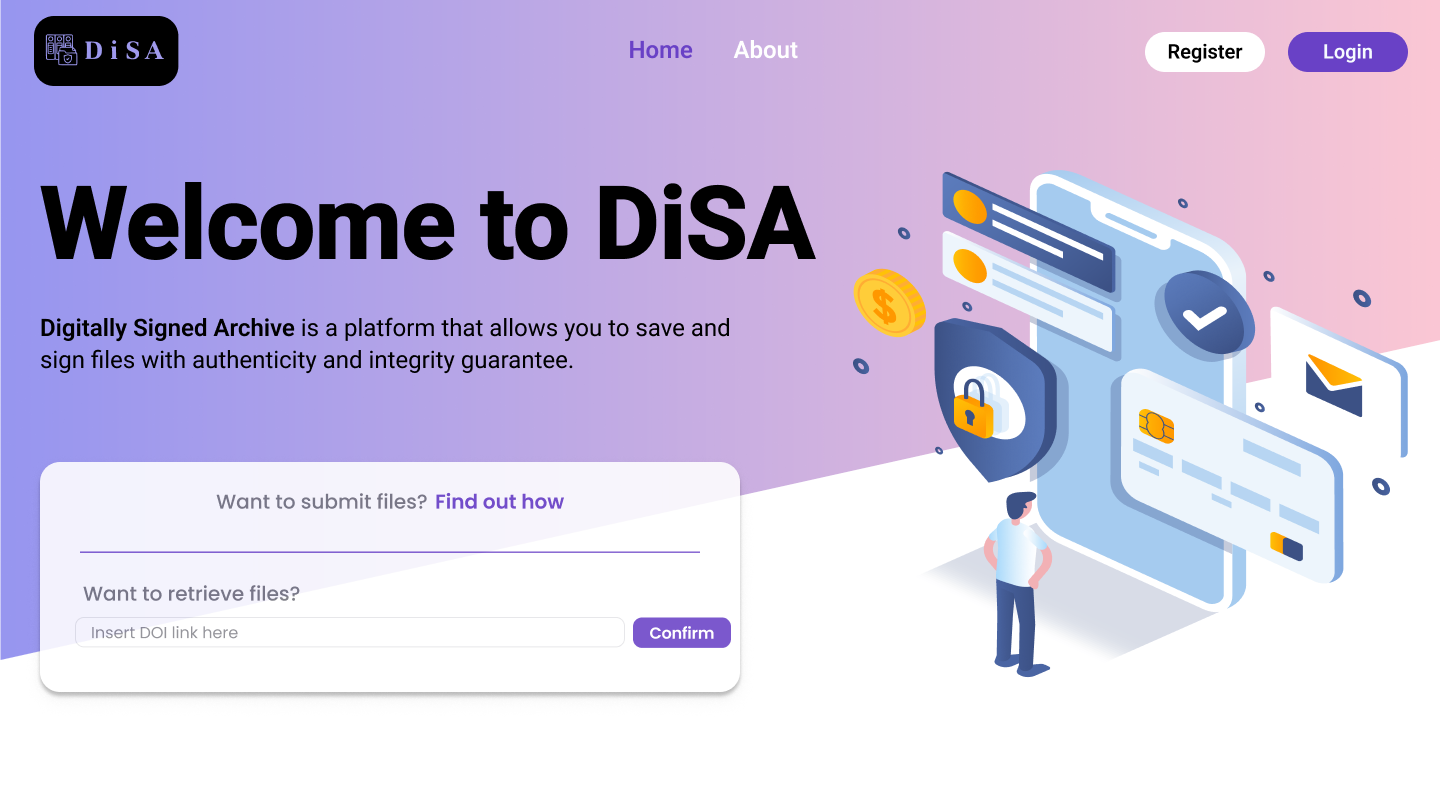
\includegraphics[width=0.8\linewidth]{images/Landing Page.png}
                        \caption{Home Page}
                        \end{figure}

                        \begin{figure}[htbp]
                        \centering
                        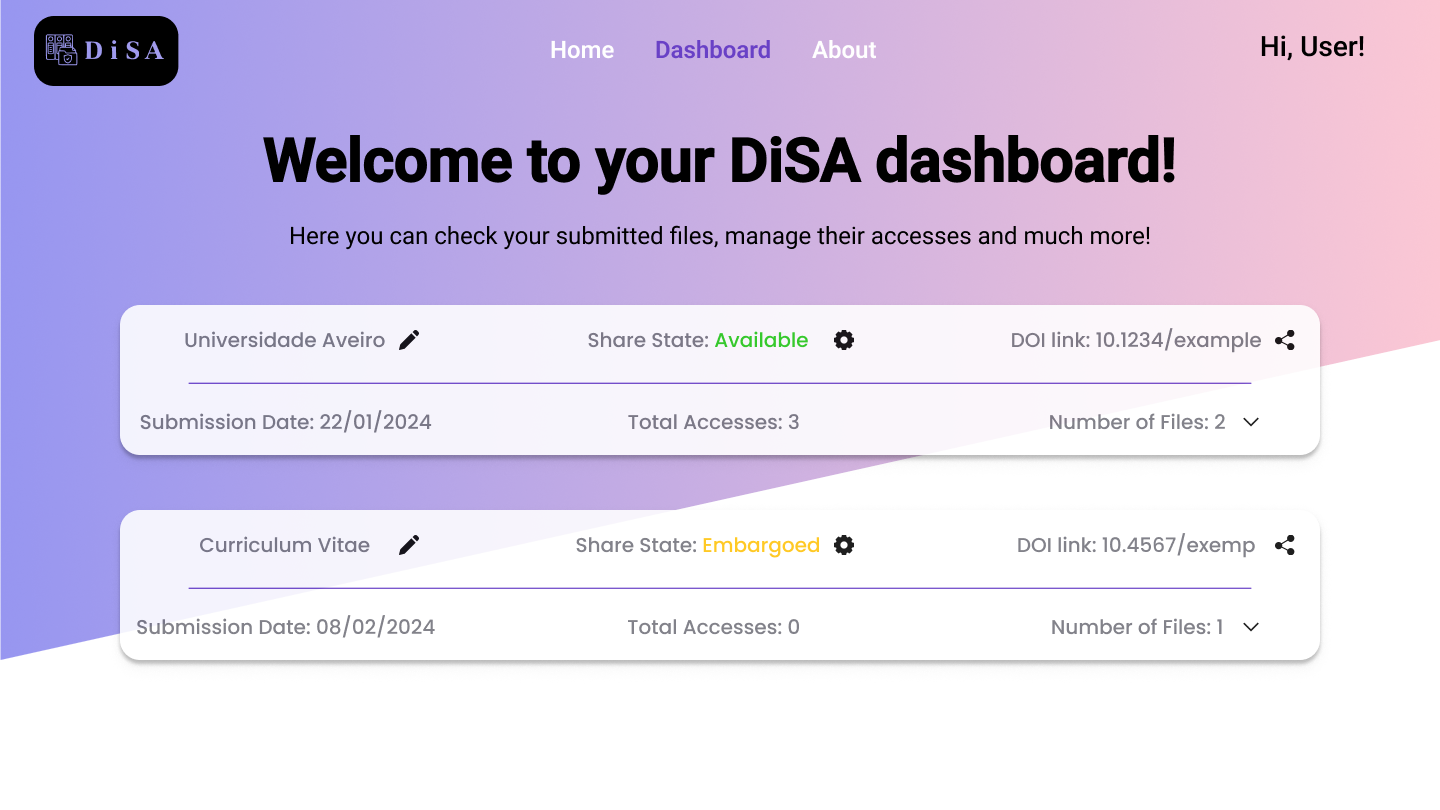
\includegraphics[width=0.8\linewidth]{images/Dashboard Page.png}
                        \caption{Dashboard - Collection Overview}
                        \end{figure}

                        \begin{figure}[htbp]
                        \centering
                        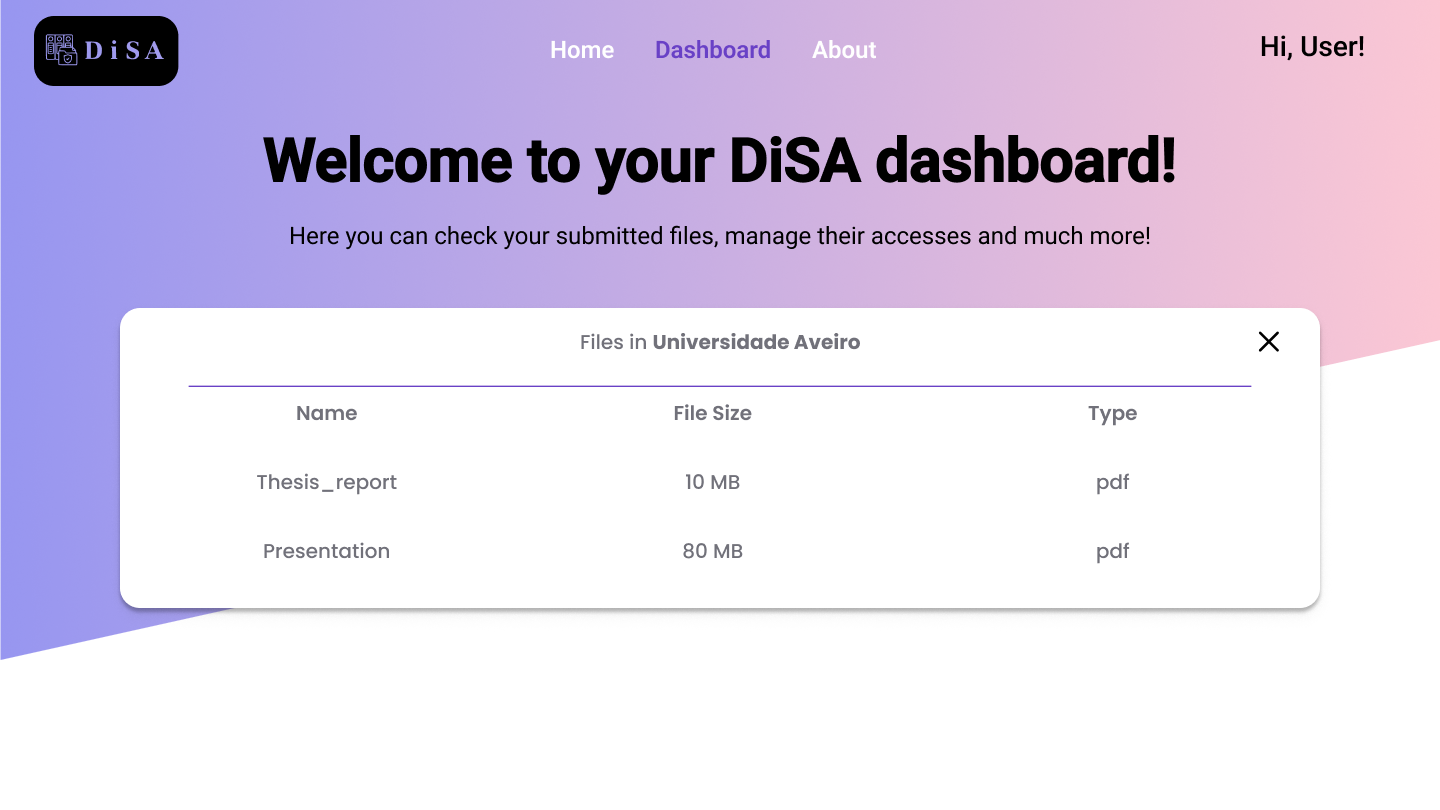
\includegraphics[width=0.8\linewidth]{images/Dashboard Page Expanded.png}
                        \caption{Dashboard - Collection Details}
                        \end{figure}

            \pagebreak
            \subsubsection{Brainstorming and Feedback}
                \quad The brainstorming sessions encouraged us to generate ideas and solutions collaboratively, the same way as feedback obtained from the course teachers changed the course of our development. Below there are some outcomes of these sessions and feedback content:
                \begin{itemize}
                    \item \textbf{Integration with External Systems:}
                    \begin{itemize}
                        \item \textbf{Objective:} Identify and assess external systems that could be integrated to enhance the functionality of DiSA.
                        \item \textbf{Results:} Initially, we considered using Archivematica for archiving, but due to technical issues, we opted for Paperless. Additionally, we integrated Autenticação.gov for user authentication as well as signatures and Polygon PoS for blockchain timestamps.
                    \end{itemize}
                    The final result is viewable in the architecture (Figure\ref{architecture}).
        
                    \item \textbf{Authentication Methods:}
                    \begin{itemize}
                        \item \textbf{Objective:} Explore different authentication methods to ensure security and usability.
                        \item \textbf{Results:} We decided to implement authentication via Autenticação.gov due to its robustness and acceptance by public institutions (in the country we live, Portugal). We also discussed the possibility of adding a login with our University's Identity Provider, but that would restrict our audience even more adding to the fact that it does not support document signatures.
                    \end{itemize}

                    \pagebreak
                    \item \textbf{Integration with Blockchain:}
                    \begin{itemize}
                        \item \textbf{Objective:} Utilize blockchain technology to ensure document integrity and authenticity over time.
                        \item \textbf{Results:} We implemented integration with Polygon PoS to provide immutable timestamps. This ensures that documents cannot be altered without leaving a trace, increasing users' trust in the integrity of the files.
                    \end{itemize}
                
                    \item \textbf{Adding GUI for Client-Side App:}
                    \begin{itemize}
                        \item \textbf{Objective:} Develop a graphical user interface (GUI) for the client-side application, making it easier for users to interact with the system.
                        \item \textbf{Results:} We created an intuitive GUI that allows users to submit documents, verify their authenticity, and manage files efficiently. This decision was made after negative feedback from potential users having to work with a command line interface.
                        \item \textbf{Image of the developed GUI:}
                        \begin{figure}[htbp]
                        \centering
                        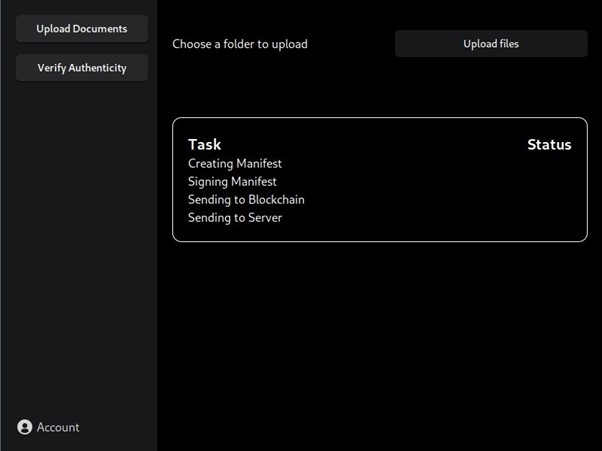
\includegraphics[width=0.8\linewidth]{images/client-side app.jpg}
                        \caption{Client-side app} 
                        \end{figure}
                    \end{itemize}
                \end{itemize}

            \pagebreak
            \subsubsection{Dependencies and Risks}
            \quad Considering the knowledge we have acquired in this bachelor's degree, even though this will not be a system launched into production we still decided to summarize the effects of dependencies and risks in a slightly closer to real-world scenario.
                \begin{itemize}
                    \item \textbf{Technology Dependencies:}
                    \begin{itemize}
                        \item \textbf{Risk:} Dependency on third-party technologies and libraries may lead to compatibility issues or unexpected changes in functionality.
                        \item \textbf{Mitigation:} Regularly update, monitor dependencies and conduct compatibility testing, and have contingency plans in place for alternative solutions.
                        \item \textbf{Contingency Plan:} A way to avoid the platform being compromised would be to go for a modular approach, so that we could add or replace any archive system, authentication or integration service.
                    \end{itemize}
                    \item \textbf{Security Risks}
                    \begin{itemize}
                        \item \textbf{Risk:} Vulnerabilities in the system's security architecture could lead to data breaches, unauthorized access, or manipulation of documents.
                        \item \textbf{Mitigation}: Implement robust security measures, including access controls, encryption, and regular security audits to identify and address potential vulnerabilities.
                    \end{itemize}
                \end{itemize}

                 \textbf{Note:} Some security measures are dependent on services (e.g. Multi-Factor Authentication is a standard in Autenticação.gov), besides this, as this project is not to be launched into production, regularly updating dependencies and auditing system behaviour is not nearly has important, yest still something to consider.
        
        \subsection{System Architecture}
            \quad DiSA's system architecture is made of various components and layers that work together to facilitate document management, authentication and preservation which will be discussed below.
        
            \subsubsection{Domain Model}
                \quad   DiSA's Domain Model represents the conceptual framework of the system, defining entities and their relationships. Key entities include:
                \begin{itemize}
                    \item \textbf{User:}: Represents individuals or organizations using the system for document management.
                    \item \textbf{Document:} Represents digital documents submitted to the system for storage and preservation.
                    \item \textbf{Blockchain:} Represents the underlying blockchain technology used for document time-stamping and authentication.
                    \item \textbf{Authentication Provider:} Represents the external service/mechanism used for user authentication.
                \end{itemize}
                
            \subsubsection{Architecture Design}
                \quad DiSA's architecture follows a modular and scalable approach, comprising several layers (limitations discussed in Section \ref{sec:limitations}):
                \begin{figure}[htbp]
                    \centering
                    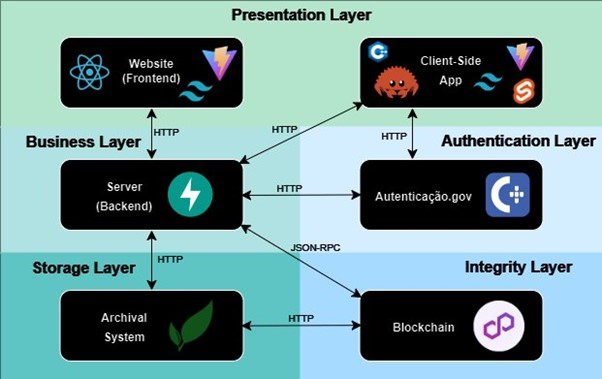
\includegraphics[width=\linewidth]{images/Architechture.jpeg}
                    \caption{DiSA's Architecture}
                    \label{architecture}
                \end{figure}
                
                \begin{itemize}
                \item \textbf{Presentation Layer (front-end):} Website and Client-Side App
                
                    This layer is responsible for all user interface components, including the web interface and client-side application. It handles user interactions, presenting data from the system to the user and collecting input from the user to send to the back-end.
        
                \item \textbf{Business Layer (back-end):} Server
                
                    This layer implements the core business logic and functionality of the system. It processes document submissions, manages verification procedures, handles document retrieval requests, and performs other document management operations.
                    
                \item \textbf{Storage Layer (database):} Archival System
                
                    This layer is responsible for the storage and retrieval of digital documents. It includes databases and file storage systems for maintaining document metadata and content, ensuring that documents are securely stored and easily retrievable.

                \item \textbf{Authentication Layer:} Autenticação.gov
                
                    This layer manages user authentication and digital signatures. It verifies user credentials and enforces security policies to ensure authorized access to the system resources. Additionally, it provides each set of documents an authentic signature.
        
                \item \textbf{Integrity Layer:} Blockchain
                    
                    This layer ensures the integrity of documents using blockchain technology. It provides mechanisms for document time-stamping and tamper detection, thereby maintaining the trustworthiness of archived documents.

                \end{itemize}
                
            \subsubsection{Deployment}
                \quad In order to facilitate future deployments, the project sub modules (excluding the client-side signing app, which isn't meant to be deployed) were turned into Docker containers in order to abstract from the deployment environment.

    \clearpage
    \section{Implementation}\label{sec:implementation}
        \quad In this section the various architecture layers will be discussed in detail, referring technologies and techniques used while implementing the idealized product.
        
    \subsection{Presentation Layer}
        \quad Starting with the presentation layer, as seen in the architecture diagram (Figure \ref{architecture}), there are a total of two user interfaces in our system: the client-side app and the web interface. These interfaces serve different purposes and cater to various user needs.
        
        The client-side app is designed for file submission, particularly for accessing USB ports which browsers typically cannot access. The web interface provides a more user-friendly experience, facilitating user interactions and enabling login through the selected authentication technology.

       \subsubsection{Client-side App}
            \quad The client-side application of DiSA comprises a comprehensive tool-set designed for indexing, signing, and storing documents in a blockchain, as well as interacting with a remote server. The client-side app is divided into several components, including a CLI (Command Line Interface), a GUI (Graphical User Interface), and a shared library.
            
            \vspace{0.25cm}\textbf{Project Structure}
            
            The project is organized as follows:
            \begin{itemize}
                \item \textbf{CLI:} Contains the source code for the command line interface.
                \item \textbf{sig\_lib:} Contains the source code for the shared library used by both the CLI and the GUI.
                \item \textbf{src-tauri:} Contains the source code for the Tauri \cite{Rust} Rust files which are integral to the GUI.
                \item \textbf{src:} Contains the source code for the GUI interface.
            \end{itemize}
            
            \vspace{0.25cm}\textbf{Development and Build Process}
            
            The development of the client-side app utilizes Rust for core functionalities and Tauri for the GUI, chosen for its compatibility with web technologies necessary for integrating with the Autenticação.gov authentication API. The development environment requires both Rust and C++ tool-chains, as well as Node.js \cite{NodeJs} or Bun \cite{Bun} for the GUI development.
            
            \begin{itemize}
                \item \textbf{CLI Development:} Developed using the Clap \cite{Clap} library in Rust, it provides functionalities for indexing directories, generating hashes, signing them, and optionally sending files to a remote server.
                \item \textbf{GUI Development:} Developed using Tauri, which integrates web technologies with Rust. It requires setting environment variables and has dependencies on specific system configurations and libraries.
            \end{itemize}
            
            \vspace{0.25cm}\textbf{Environment Configuration}
            
            The application requires a `.env` file to store environment variables, which should be placed at the root of either the CLI or GUI application directories. Key environment variables include the release mode, where development skips the signature part and production does not, also authentication variables to be used with the Digital Mobile Key server and blockchain variables for its interactions.
            
            \vspace{0.25cm}\textbf{Building and Running}
            
            The client-side app can be built and run in both development and production modes. Pre-compiled binaries for Windows and Linux are available for easier deployment. Ensure all dependencies and environment variables are correctly configured for proper functionality.
            
            \vspace{0.25cm}\textbf{Installation and Deployment}
            
            Pre-compiled binaries are available but may not interact with the server or produce valid signatures. Proper configuration of environment variables is crucial for successful deployment.
            
            \vspace{0.25cm}\textbf{Known Issues and Troubleshooting}
            
            The project includes a FAQ section to help troubleshoot common issues, such as compilation errors and environment setup problems. Key issues include compilation issues, card reader detection and GUI display issues.
            
        \subsubsection{Web Interface}
            \quad For the web interface, we developed a React-based website using Tailwind CSS \cite{Tailwind} for styling and Vite \cite{Vite} as the build tool. The main reason for developing this component was to create an easily maintainable and interactive part of our project, allowing less tech-savvy users to navigate our system and perform their desired operations seamlessly.
    
            \vspace{0.25cm}\textbf{Design and layout}
            
            To ensure an intuitive design, we started by sketching some mock-ups using Figma as see above in Section \ref{sec:mockups}. This step was crucial for visualizing the user flow and interface elements before actual development. Once the design was finalized, we proceeded with the development using the planned technologies.
            
            \vspace{0.25cm}\textbf{Data presentation and visualization}
            
            These are critical for users to understand and interact with their documents effectively. Our approach includes:
            \begin{itemize}
                \item Visual Cues: Icons and color codes are used to indicate the status and actions available for each collection of documents.
                \item Interactive Elements: Users can interact with elements such as links and buttons to perform actions like downloading or verifying documents.
            \end{itemize}
            
            \vspace{0.25cm}\textbf{Error report and feedback}
    
            Providing users with clear feedback and error reporting is essential for a smooth user experience. We implemented the following mechanisms:
            \begin{itemize}
                \item Error Messages: Informative error messages are displayed when an issue occurs, guiding users on how to resolve it.
                \item Form Validation: Real-time validation of form inputs helps prevent errors before submission.
            \end{itemize}
    
            \vspace{0.25cm}\textbf{Integration with the business layer}
    
            The presentation layer integrates seamlessly with the business layer, ensuring that all user actions are processed correctly and efficiently. This integration involves:
            \begin{itemize}
                \item API calls: The front-end communicates with the back-end through a series of API calls using the fetch API, handling data retrieval, submission and updating.
                \item Security Measures: Implementing security best practices, such as token-based authentication to protect user data and interactions.
            \end{itemize}
    
        \subsection{Authentication Layer}
            \quad The Authentication Layer plays a crucial role in ensuring that only authorized users can access the DiSA system. It encompasses mechanisms for verifying the identity of users and granting them access based on their roles and permissions.
            
        \subsubsection{User Authentication}
            \quad The system primarily leverages the robust and secure authentication provided by Autenticação.gov. This authentication method offers reliable identity verification through government-issued credentials and implements two-factor authentication (2FA), enhancing the overall security of the system. Additionally, DiSA offers conventional login functionality due to constraints in our project and easiness in developing scenarios. More is discussed in (Section \ref{sec:limitations}).
            
        \subsubsection{Access Control}
            \quad Access control in DiSA is managed using JSON Web Tokens (JWT) \cite{JWT}, which serve as bearer tokens for authenticating users and authorizing their access to system resources. Most requests to the system endpoints require a valid JWT token for authentication and authorization purposes. However, there is an exception for accessing shared collections, where access is granted without the need for a user account within the system. This approach ensures secure access to sensitive data while facilitating seamless collaboration and data sharing among users, even if they are not registered users of the system.
        
        \subsection{Business Layer}
            \quad For the Business Layer, we implemented a robust and scalable architecture using FastAPI, a modern and efficient web framework. We leveraged its features to create a robust and scalable API that handles the business logic.
            \subsubsection{Integration with Services}
                \quad The Service Integration layer is responsible for communicating with the storage services. The Paperless-ngx service was chosen due to it's specialized focus on handling textual documents.  
            
        \subsection{Storage Layer}
            \quad For our storage layer, we used the SQLModel \cite{SQLModel} package, which integrates natively with FastAPI's \cite{FastAPI} data validation model. This allowed us to use the same baseline model to create models for API validation, response and also the database schema. 
    
            SQLModel uses the SQLAlchemy Object-Relational Mapper (ORM) \cite{SQLAlchemy}, integrating it with the Pydantic validation library \cite{Pydantic}. For our database, we chose to go with SQLite \cite{SQLite} as it simplified our development, while also not damaging future DB migration efforts.
            \subsubsection{Database Design}
                \quad As said above, our database definition is somewhat influenced by the joint validation-definition baseline model. Regardless, we chose to use the database purely as a data store. We believe that this leads to a better separation of concerns, while also greatly benefiting the developer experience.
                
            \begin{figure}[htbp]
                \centering
                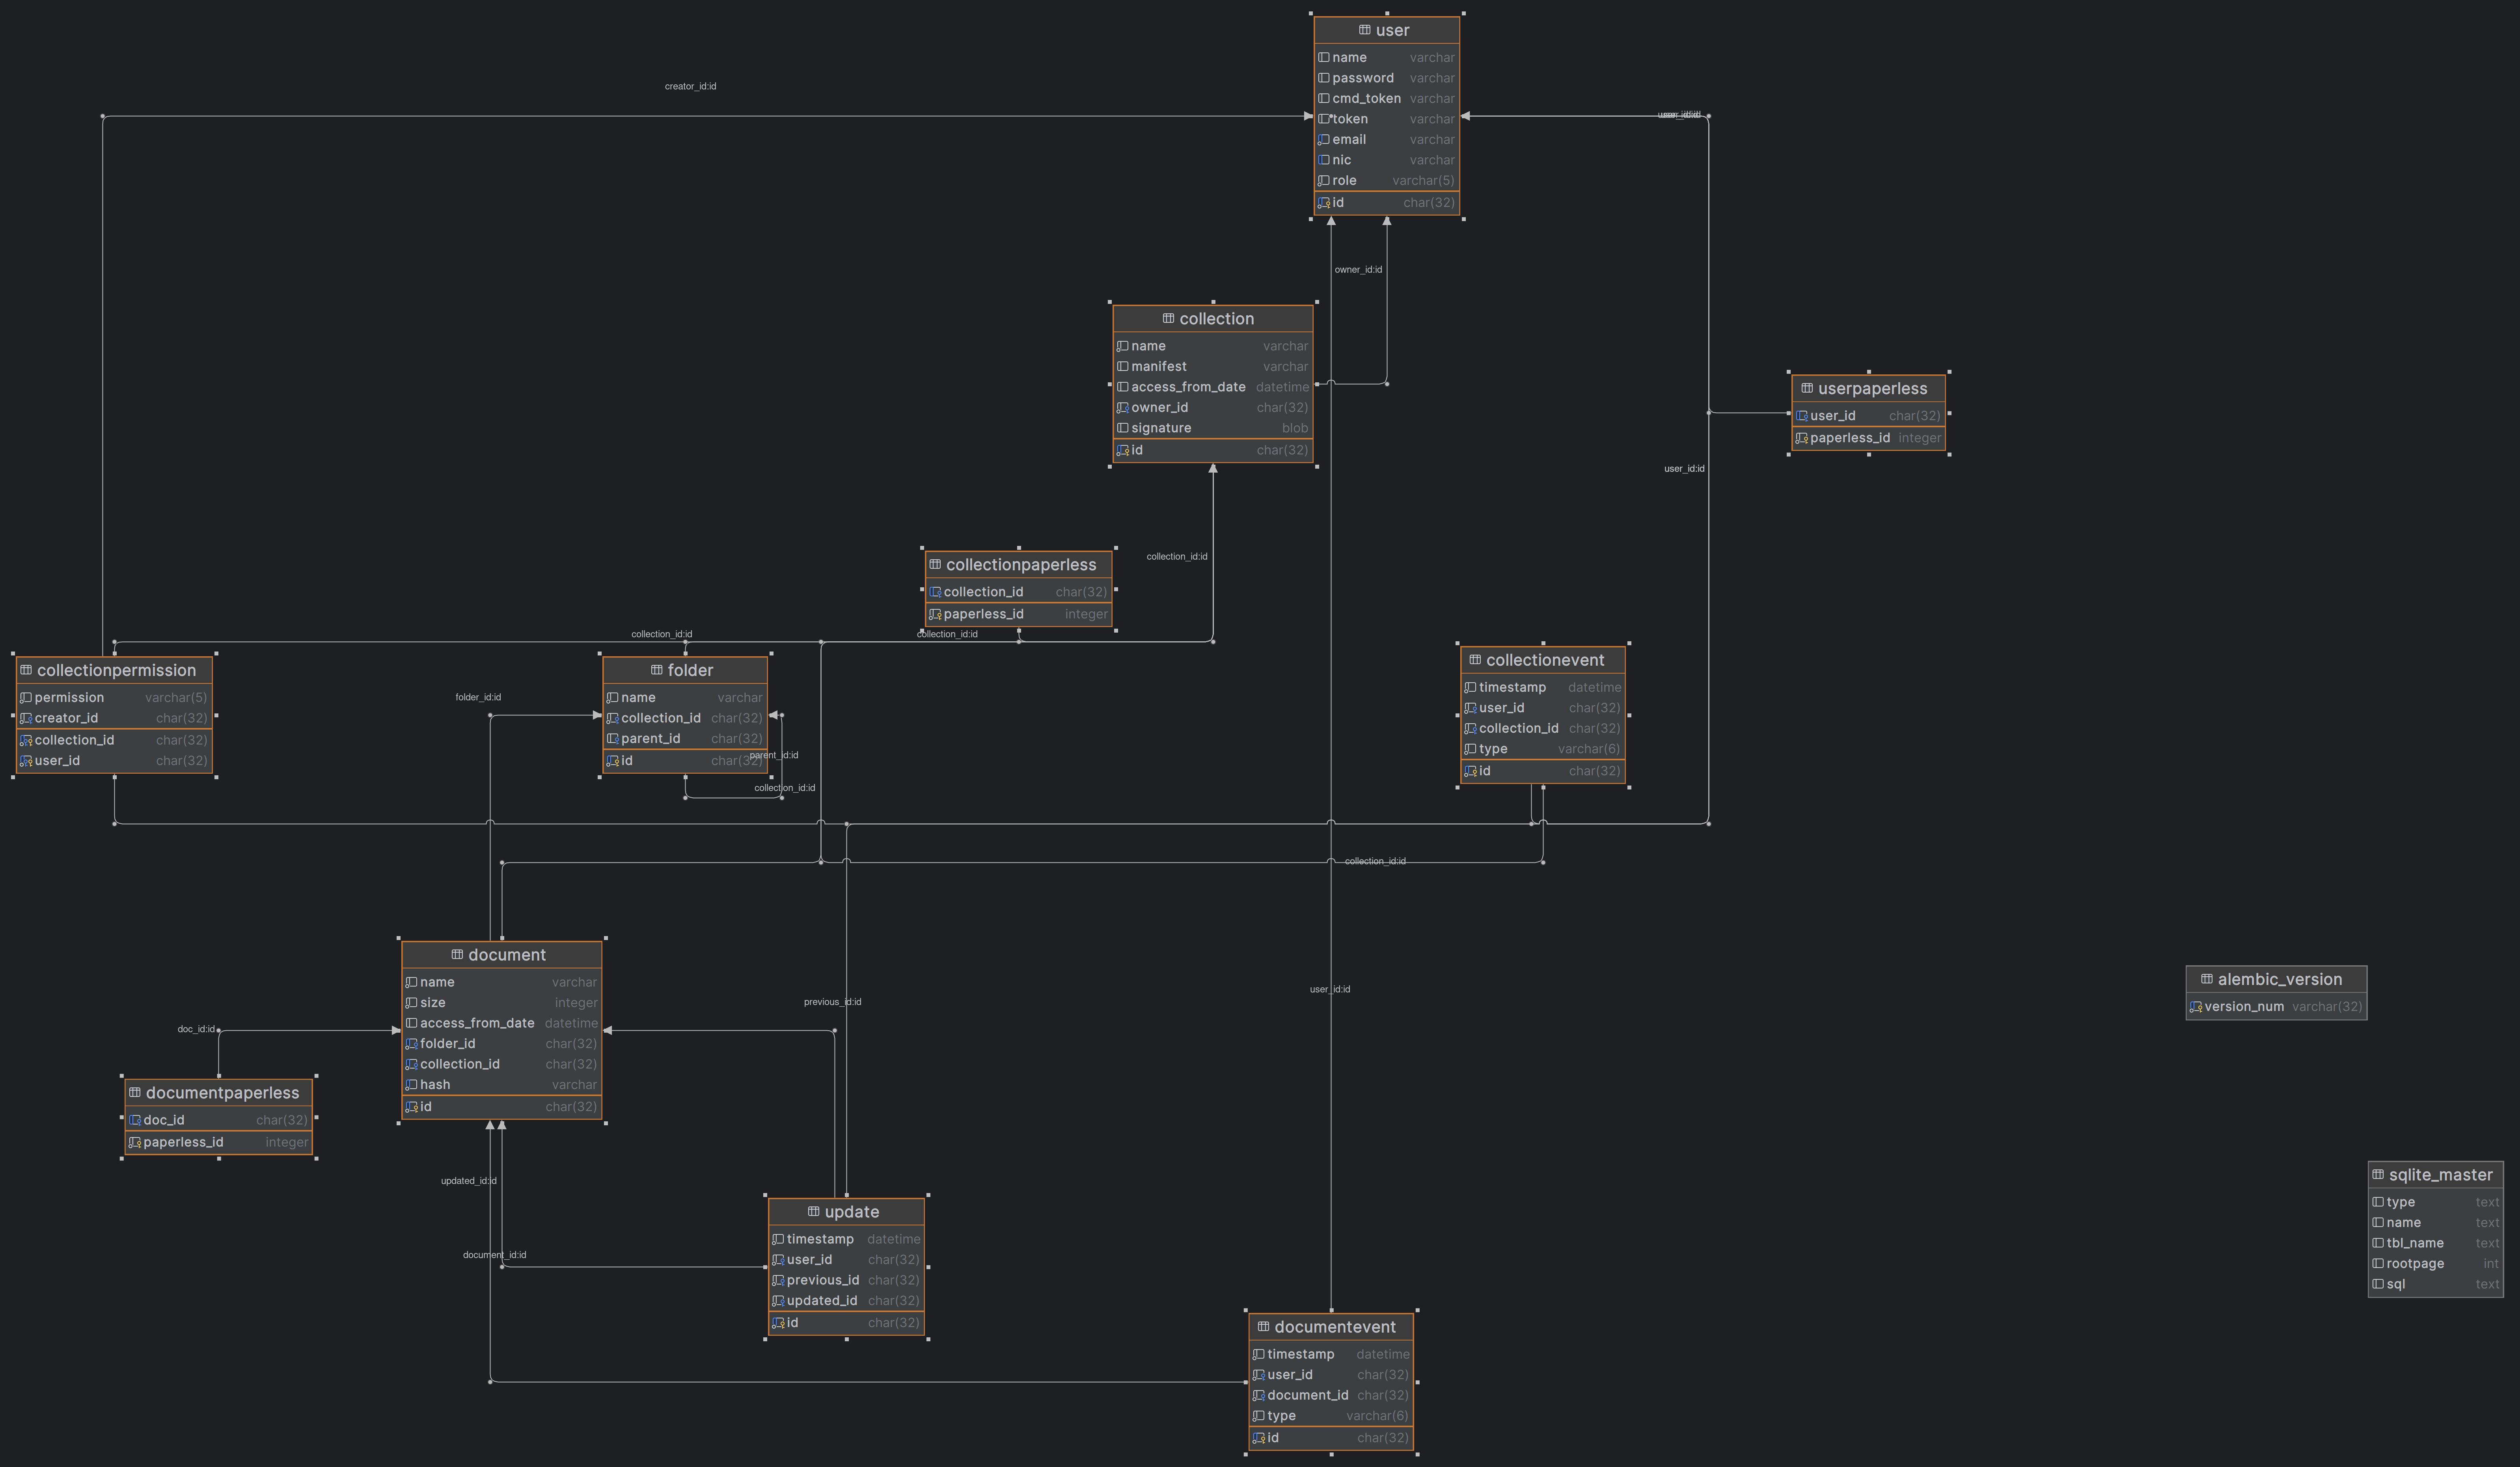
\includegraphics[width=\linewidth]{images/Database Design.jpg}
                \caption{Database Design}
            \end{figure}
            \subsubsection{Database Management}
                \quad As we use SQLite for our DB system, we can skip using a dedicated DBMS and for our migrations, we chose to go with Alembic. It is a package designed by the developer of SQLAlchemy, with the goal of simplifying migrations.
        
        \subsection{Integrity Layer}
            \quad \textbf{Blockchain definition:} At its base, a blockchain is a chain of transactions that aims to guarantee their authenticity via a mechanism of chained signatures.
                
            \quad Whenever a new transaction occurs (regardless of whether or not tokens are exchanged), the owner must sign both the hash of the previous transaction and the recipient's (in this case, the smart contract's) public key and add it to the end of the transaction. \cite{bitcoin}
                
                \subsubsection{Authenticity Verification} 
                    \quad Since every transaction's signatures are linked together this way, in order to alter a transaction that was already inserted in a blockchain, a malicious actor must gather not only the transaction owner's private key, but also the private keys from everyone that inserted a transaction before, which, in the case of public networks like Polygon (which had gained 15.24 million users just in 2023 alone \cite{polygonUserCount}), is virtually impossible.
                        
                    \quad As such, blockchains become the ideal mechanism for guaranteeing our document's validity, and since blockchains become more secure the more popular they are (as well as the cost and difficulty of hosting one ourselves) we opted to deploy our smart contract\footnote{\textbf{Smart Contract}: objects that exist in the blockchain and that allow us to execute actions (like storing hashes) automatically} in the Polygon PoS blockchain. 
            
                \subsubsection{Downsides of using a blockchain} 
                    \quad The one downside of using a blockchain, is that, unless you're testing, you'll have to pay a gas fee, however by storing only the manifest's hash, we managed to cut down data costs to the point where, at the current rate, a single dollar is enough for approximately 2000 transactions.
    
    \clearpage
    \section{Project Management}
        \quad Effective project management is essential for the successful development and deployment of any project, including our own, DiSA.
        
        \subsection{Team Roles}
            \quad We distributed roles across our team considering their experience in each component of the overall system, allowing for the project outcomes to flow in an optimized way.
            \begin{itemize}
                \item \textbf{André Cardoso:} Team Leader 
                \item \textbf{Bruno Páscoa:} Architect 
                \item \textbf{Maria Sardinha:} Back-end Developer 
                \item \textbf{Miguel Pinto:} Front-end Developer 
                \item \textbf{Pedro Rei:} Developer 
                \item \textbf{Tiago Figueiredo:} DevOps Master 
            \end{itemize}
                
        \subsection{Communication Plan}
            \quad Along with proper work distribution, effective communication is crucial.
            \begin{itemize}
                \item \textbf{Main Repository:} 
                \begin{itemize}
                    \item \href{https://github.com/Mycsina/DiSA/}{GitHub} for version control and collaborative development. It is made of sub-modules representing each component.
                \end{itemize}
                \item \textbf{Documentation website:}
                \begin{itemize}
                    \item \href{https://agh4m.github.io/PI-SITE/}{GitHub} for overall view of our system's features, deliverables and team.
                \end{itemize}
                \item \textbf{Within Group:}
                \begin{itemize}
                    \item \textbf{Meetings:} As needed via Discord.
                    \item \textbf{Conversations:} Daily communications via WhatsApp group.
                    \item \textbf{GitHub Issues and Pull Requests:} Feature description and status by submitting issues or creating pull requests on each corresponding GitHub repository.
                \end{itemize}
                \item \textbf{With the Advisors:}
                \begin{itemize}
                    \item \textbf{Meetings:} Scheduled once per week (more if needed) via Zoom.
                    \item \textbf{Conversations:} As necessary via email, managed by the group representative (André Cardoso).
                \end{itemize}
            \end{itemize}
            
        \subsection{Project Schedule}
            \quad Our project schedule adapted to key milestones, deliverables, and timelines for the DiSA project, following the OpenUP methodology. It includes the following phases:
            \begin{itemize}
                \item \textbf{M1 - Inception} 
                
                During the Inception phase, we defined the project's scope, objectives and high-level goals by discussing the project proposal with our advisors and between team members. We also started thinking of where to find similar work to our proposal and defined our communication plan.

                \item \textbf{M2 - Elaboration}

                Along the Elaboration phase we deepened our requirements gathering process and consulted an experient user of an archival platform, Rafael Direito, which has experience with Archivematica (our initial proposal as archival system). Also we developed initial views for our system's architecture, information flow as well as actors, use-cases and design mockups.

                \item \textbf{M3 - Construction}

                In the Construction phase the team actively developed the idealized features, with focus on having the biggest progress along the information flow. Some of the implemented features involved blockchain integration, document storage (limited to meta-data), digital signatures and CLI release.
                
                \item \textbf{M4 - Transition}

                The Transition phase was remarked by the development of remaining key features as document storage (whole documents), document sharing, login using Autenticação.gov. In addition, recognizing our platforms state, limitations, possible challenges when considering a real-world scenario as well as future work.
                
            \end{itemize}
            \quad The project schedule was continuously monitored and adjusted as needed to adapt the changing requirements, resource constraints, and external dependencies. This was most noticeable upon our change of archival system between M3 and M4 from Archivematica to Paperless.

    \clearpage
    \section{Conclusions and Future Work}\label{sec:conclusionsfuturework}
        \quad In this section we present what were the overall outcomes upon developing DiSA, as well as its implemented features, limitations, change of plans compared to previously planned ideas or features being our own or part of the project's proposal, and possible future work were this system meant to go to production.

        \subsection{Main Results}
            \quad The development of the DiSA project has culminated in the creation of a new platform for digital document management and authentication. Key achievements and main results include:
            \begin{itemize}
                \item \textbf{Comprehensive Solution:} DiSA is able to provide individuals and organizations with a comprehensive solution for secure, authentic, and long-term document management. By integrating digital signatures and blockchain technology, DiSA ensures the integrity and authenticity of digital documents while offering scalable storage and seamless access.
                \item \textbf{User-Centered Design:} The user interface and experience of DiSA are designed with a focus on usability, accessibility, and efficiency. Intuitive features and functionalities streamline document submission, retrieval, and sharing, enhancing user satisfaction and engagement.
                \item \textbf{Technological Innovation:} DiSA leverages advanced technology such as blockchain and digital signatures to deliver good document-manage capabilities. By harnessing the benefits of these technologies, DiSA sets new standards for document authenticity and security.
            \end{itemize}

        \subsection{Implemented Features}
            \quad Throughout the semester, our group successfully developed and implemented several key features that make DiSA a robust and user-friendly platform for digital document management. Considering the previously mentioned requirements (Section \ref{sec:fun-requirements}) we can state that we have implemented all but with some caveats, which we will state here.
            \begin{itemize}
                \item \textbf{Document Submission:} 
                    \begin{itemize}
                        \item The system does allow for users to submit files or folders at once (1 or more files).
                        \item The system does support large file submissions.
                    \end{itemize}
                    
                \pagebreak
                \item \textbf{Authenticity Guarantee:} 
                    \begin{itemize}
                        \item The system does allow for digital signatures with citizen card or digital mobile key.
                        \item Even though the business layer allows to partially change a document collection, the web interface does not allow so for simplicity, therefore there are no changes to documents after submission at all.
                        \item The client-side app has a method to check a signature validity and both components of the presentation layer have a direct link to the blockchain service used where the receipt hash (manifest) can be seen to be the same.
                        \end{itemize}
                        
                \item \textbf{Proof of Existence:} 
                \begin{itemize}
                    \item The system successfully incorporated a mechanism to prove the existence of a document at a given time, by integrating a blockchain technology. 
                \end{itemize}
                        
                \item \textbf{Document Sharing:} 
                \begin{itemize}
                    \item The system does generate a unique link, but it is done so in the web interface, taking advantage of the collection's UUID, not a Digital Object Identifier (DOI) link \cite{DOI}, similarly to what was part of the project's proposal.
                \end{itemize} 
                    
                \item \textbf{Persistence Archive:} 
                \begin{itemize}
                    \item The system does have integration with an archival platform by an adapter, allowing for more and different platforms to be added or removed as required.
                \end{itemize}
                        
                \item \textbf{User Interface:} 
                \begin{itemize}
                    \item The system does have a minimalist user interface with what we consider self-explainable steps, but due to time constraints there were no usability test performed to prove so.
                \end{itemize}
                        
                \item \textbf{Receipt Generation:} 
                \begin{itemize}
                    \item The system does generate a receipt, which we call manifest and its hash is what is submitted to the blockchain and used to prove document's integrity and existence, yet it does not link the original document, as there is no additional process after document submission, besides compressing them to a \textit{.tar} file.
                \end{itemize}
            \end{itemize}

        \subsection{Limitations}  \label{sec:limitations}
            \quad As outcomes of the development of DiSA there are some limitations and areas for improvement that need to be addressed:
            
            \begin{itemize}
                \item \textbf{Documentation:} The documentation for DiSA could be adjusted in a more detailed and structured way to guide mainly end-users and also developers in understanding and utilizing the system effectively. This includes user guides, API documentation, and troubleshooting manuals.
    
                \item \textbf{Coding Convention:} The code-base of DiSA lacks standardized coding styles and conventions. This inconsistency can lead to difficulties in maintenance and collaboration among developers. Adopting a standardized coding style and implementing code reviews would improve code quality and maintainability.
    
                \item \textbf{Testing:} The testing of DiSA was limited primarily to inter-team testing of endpoints to verify basic workflow functionality. Comprehensive testing practices, such as static code analysis, prototype testing, and functional testing, were not implemented. While initial tests confirmed the system's basic operations, further rigorous testing is necessary to ensure reliability, performance, and security.
    
                \item \textbf{Incomplete Functionality:} The web interface does not fully exploit the back-end functionalities. While the back-end supports a wide range of features, many of these are not yet integrated into the web interface, limiting the user's ability to leverage the full capabilities of DiSA through the web platform. Namely peeking into a collection's files, having a detailed view of its events (e.g. document updates and accesses).
    
                 \item \textbf{DOI Links:} The system currently does not utilize DOI (Digital Object Identifier) links as initially proposed. Due to imposed payment and partnership with institutions managing said links and the fact that there was no funding to achieve said partnerships the integration of DOI links was not feasible. This limits the system's ability to provide unique, persistent links for digital documents, which could impact document traceability and citation.
    
                \item \textbf{Login with Digital Mobile Key:} The login with Digital Mobile Key (CMD) is currently implemented only in a pre-production environment. The full production version of this feature requires payment, which was not feasible due to the lack of funding for this project. As a result, the system does not fully support CMD login for real-world use, which limits its applicability for users who rely on this authentication method, thus there is a standard email and password login in the final result.
            \end{itemize}

        \subsection{Real-world challenges}
            \quad While DiSA represents an advancement in digital document management, there are some challenges to deal considering a real-world scenario:
            \begin{itemize}
                \item \textbf{Scalability Challenges:}
                DiSA's scalability may be constrained by external factors, mainly the third-party services chosen:
                \begin{itemize}
                    \item The authentication method used (Autenticação.gov) is restricted to Portugal, as it was developed to be a national service, therefore it imposes a challenge in case DiSA was intended to be published to a broader audience.

                    \item Depending only on one archival system could bring consequences, due to the possibility of at a certain point said system not be sufficient for our platform's needs.

                    \item We never tested the system with high transfer loads and concurrent access, but in a real-world scenario it would be necessary to improve its efficiency handling such situations, as reliability is a key aspect of an archival system.
                \end{itemize}.
                 
                \item \textbf{Integration Complexity:} Integrating DiSA with existing systems, especially those with complex configurations, may pose more challenges. 
                \begin{itemize}
                    \item In an attempt at solving or preventing scalability issues, we may face complexity issues by having integrated too many third-party services (e.g. having to manage dozens of archival platforms is both an intensive task in software and real-world terms, as deals with said systems may change).

                    \item Integrating country specific dependencies will also bring high complexity levels, as for example, the chosen signature service is well known and trusted in Portugal it might be true for other services in other countries or regions.

                    \item Accepting new standards will also be a challenge, as technology evolves, new cipher algorithms may arise, as old ones are exploited, plus integrating 
                \end{itemize}
                
                \item \textbf{User Adoption:} 
                \begin{itemize}
                    \item User adoption of DiSA may face hurdles, particularly in organizations accustomed to legacy systems or paper-based processes. 
                    
                    \item Reliance on regional services, like Autenticação.gov, could introduce additional barriers to adoption, especially for organizations outside of Portugal. Continued user education and outreach efforts are essential to address these challenges and maximize the adoption of DiSA.
                \end{itemize}
            \end{itemize}
        
        \subsection{Conclusions}
            \quad In conclusion, the DiSA (Digitally Signed Archive) project, has successfully developed a good minimum viable product when it comes to a creation of a digital document archive with authenticity guarantee, as initially proposed by our advisors.
             
            \quad While there are limitations and real-world challenges to overcome, the potential benefits of DiSA are notable, in a way that a platform similar to ours certainly (according to us) has a place in the future paving the way for improved efficiency, transparency, and trust in digital document management processes.

            \quad As students, throughout the endeavor of developing this platform, we have gained valuable insights and experiences that resonate with the principles and teachings of our university course in Informatics Engineering by applying the knowledge and skills acquired during our studies. Concepts learned in the course, such as database management, software engineering, system architecture and cybersecurity, were essential in shaping the design and development of DiSA, as have the principles of problem-solving, critical thinking and continuous learning have also empowered us to overcome encountered challenges, making us innovate and search for solutions.

        \pagebreak
        \subsection{Future Work}
            \quad Looking ahead, we have identified several avenues for future work and enhances to DiSA:
            \begin{itemize}
                \item \textbf{Enhanced Scalability:} As previously discussed, investing in optimizations and scalability improvements to ensure that DiSA can effectively handle large volumes of documents and users is definitely a key part onto the platform's success.
                
                \item \textbf{Advanced Analytics: } Extending the developed analytics and reporting capabilities to provide users with insights into document usage, access patterns, and trends, as well as implementing mechanisms for preventing cyber-attacks, would greatly enhance the system's utility and security..

                \item \textbf{Integration with Emerging Standards:} Continuously monitoring and integrating emerging standards and technologies to ensure that DiSA remains compatible and interoperable with evolving digital document management ecosystems.

                \item \textbf{Deployment and Cloud Services:} For DiSA to be effectively utilized in a real-world setting, it should be deployed on a reliable and scalable cloud platform. This will provide accessibility, reliability, and scalability. Additionally, exploring the integration of cloud services for storage, authentication, and other functionalities can enhance the overall performance and user experience.
    
                \item \textbf{User Education and Support:} Developing comprehensive user education materials and support resources to facilitate user adoption and ensure efficient utilization of the system. This could include tutorials, FAQs, and dedicated support channels.
            \end{itemize}

    \clearpage
    \section{References}\label{sec:references}
        \printbibliography[heading=none]
        
\end{document}
